\documentclass{standalone}
\usepackage{tikz}
\usetikzlibrary{patterns, positioning}

\begin{document}
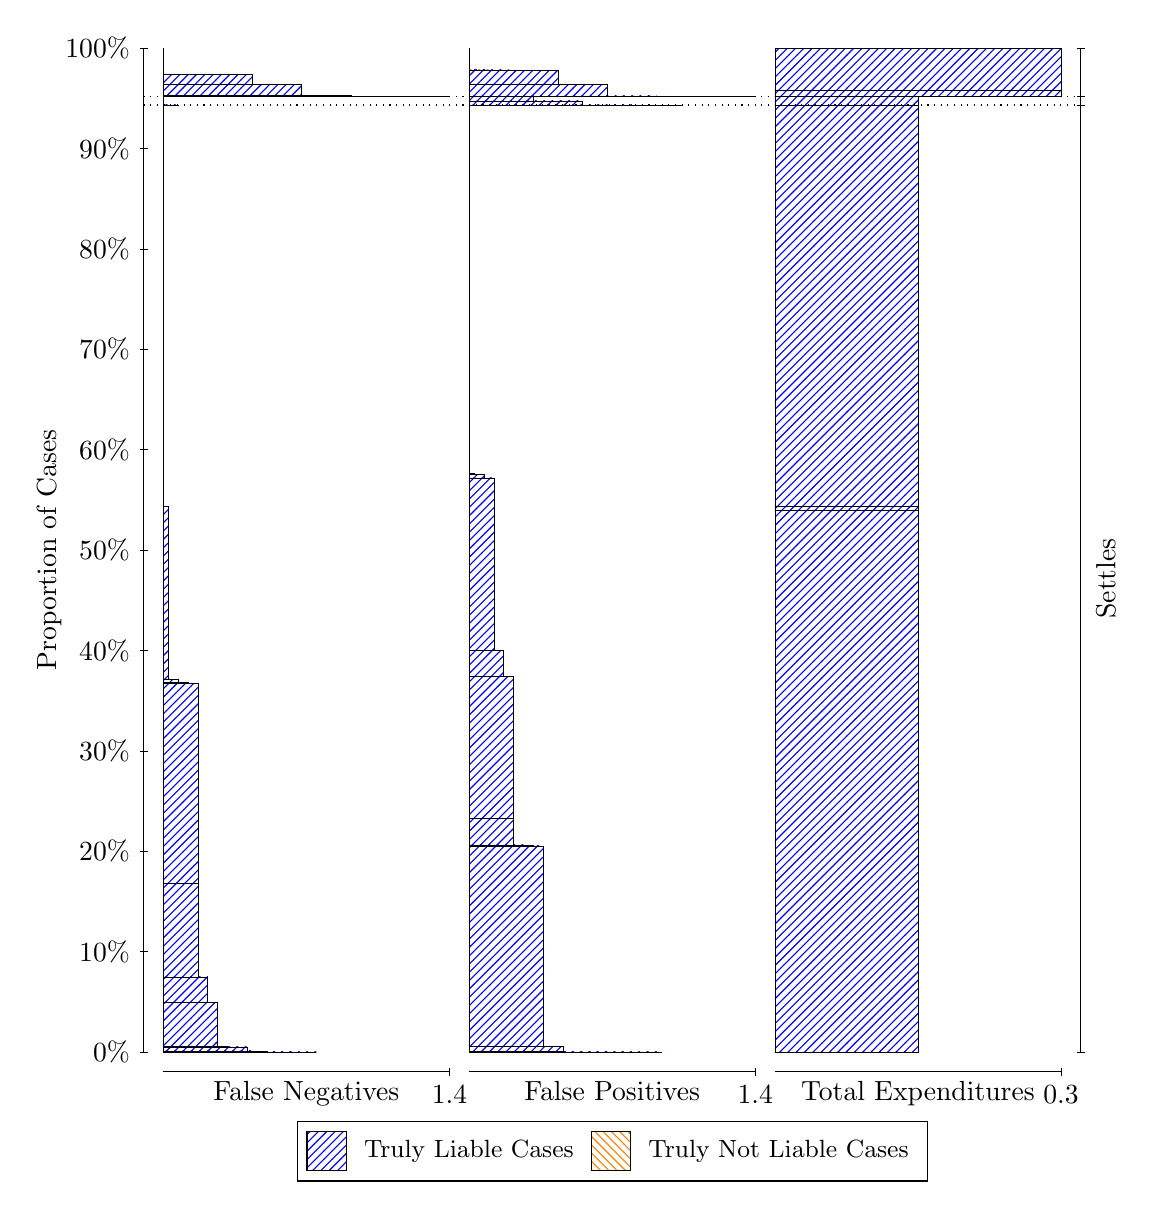
\begin{tikzpicture}
\draw[black, very thin] (1.5,1.75) -- (1.5,14.5);
\node[rotate=90, anchor=center] at (0.3, 8.125) {Proportion of Cases};
\draw[black, very thin] (1.45,1.75) -- (1.55,1.75);
\node[anchor=east] at (1.45, 1.75) {0\%};
\draw[black, very thin] (1.45,3.025) -- (1.55,3.025);
\node[anchor=east] at (1.45, 3.025) {10\%};
\draw[black, very thin] (1.45,4.3) -- (1.55,4.3);
\node[anchor=east] at (1.45, 4.3) {20\%};
\draw[black, very thin] (1.45,5.575) -- (1.55,5.575);
\node[anchor=east] at (1.45, 5.575) {30\%};
\draw[black, very thin] (1.45,6.85) -- (1.55,6.85);
\node[anchor=east] at (1.45, 6.85) {40\%};
\draw[black, very thin] (1.45,8.125) -- (1.55,8.125);
\node[anchor=east] at (1.45, 8.125) {50\%};
\draw[black, very thin] (1.45,9.4) -- (1.55,9.4);
\node[anchor=east] at (1.45, 9.4) {60\%};
\draw[black, very thin] (1.45,10.675) -- (1.55,10.675);
\node[anchor=east] at (1.45, 10.675) {70\%};
\draw[black, very thin] (1.45,11.95) -- (1.55,11.95);
\node[anchor=east] at (1.45, 11.95) {80\%};
\draw[black, very thin] (1.45,13.225) -- (1.55,13.225);
\node[anchor=east] at (1.45, 13.225) {90\%};
\draw[black, very thin] (1.45,14.5) -- (1.55,14.5);
\node[anchor=east] at (1.45, 14.5) {100\%};

\draw[black, very thin] (13.4,1.75) -- (13.4,14.5);
\draw[black, very thin] (13.35,1.75) -- (13.45,1.75);
\node[anchor=west] at (13.35, 1.75) {};
\draw[black, very thin] (13.35,13.776) -- (13.45,13.776);
\node[anchor=west] at (13.35, 13.776) {};
\draw[black, very thin] (13.35,13.886) -- (13.45,13.886);
\node[anchor=west] at (13.35, 13.886) {};
\draw[black, very thin] (13.35,14.5) -- (13.45,14.5);
\node[anchor=west] at (13.35, 14.5) {};

\draw[black, very thin, pattern color=blue, pattern=north east lines] (1.75,1.75) rectangle (3.692,1.75);
\draw[black, very thin, pattern color=blue, pattern=north east lines] (1.75,1.75) rectangle (3.4414,1.75);
\draw[black, very thin, pattern color=blue, pattern=north east lines] (1.75,1.75) rectangle (3.1908,1.75);
\draw[black, very thin, pattern color=blue, pattern=north east lines] (1.75,1.75) rectangle (3.0655,1.7605);
\draw[black, very thin, pattern color=blue, pattern=north east lines] (1.75,1.7605) rectangle (2.9402,1.7644);
\draw[black, very thin, pattern color=blue, pattern=north east lines] (1.75,1.7644) rectangle (2.8149,1.8156);
\draw[black, very thin, pattern color=blue, pattern=north east lines] (1.75,1.8156) rectangle (2.6897,1.8157);
\draw[black, very thin, pattern color=blue, pattern=north east lines] (1.75,1.8157) rectangle (2.5644,1.818);
\draw[black, very thin, pattern color=blue, pattern=north east lines] (1.75,1.818) rectangle (2.4391,2.3765);
\draw[black, very thin, pattern color=blue, pattern=north east lines] (1.75,2.3765) rectangle (2.3138,2.7029);
\draw[black, very thin, pattern color=blue, pattern=north east lines] (1.75,2.7029) rectangle (2.1885,3.8874);
\draw[black, very thin, pattern color=blue, pattern=north east lines] (1.75,3.8874) rectangle (2.1885,6.4292);
\draw[black, very thin, pattern color=blue, pattern=north east lines] (1.75,6.4292) rectangle (2.0632,6.4435);
\draw[black, very thin, pattern color=blue, pattern=north east lines] (1.75,6.4435) rectangle (1.9379,6.4857);
\draw[black, very thin, pattern color=blue, pattern=north east lines] (1.75,6.4857) rectangle (1.8126,8.6781);
\draw[black, very thin, pattern color=orange, pattern=north west lines] (1.75,8.6781) rectangle (1.75,8.6781);
\draw[black, very thin, pattern color=blue, pattern=north east lines] (1.75,8.6781) rectangle (1.75,13.776);
\draw[black, very thin, pattern color=blue, pattern=north east lines] (1.75,13.776) rectangle (1.9379,13.777);
\draw[black, very thin, pattern color=orange, pattern=north west lines] (1.75,13.777) rectangle (1.75,13.777);
\draw[black, very thin, pattern color=blue, pattern=north east lines] (1.75,13.777) rectangle (1.75,13.886);
\draw[black, very thin, pattern color=blue, pattern=north east lines] (1.75,13.886) rectangle (5.3833,13.886);
\draw[black, very thin, pattern color=blue, pattern=north east lines] (1.75,13.886) rectangle (4.7569,13.886);
\draw[black, very thin, pattern color=blue, pattern=north east lines] (1.75,13.886) rectangle (4.1305,13.899);
\draw[black, very thin, pattern color=blue, pattern=north east lines] (1.75,13.899) rectangle (3.504,14.041);
\draw[black, very thin, pattern color=blue, pattern=north east lines] (1.75,14.041) rectangle (2.8776,14.164);
\draw[black, very thin, pattern color=blue, pattern=north east lines] (1.75,14.164) rectangle (2.627,14.164);
\draw[black, very thin, pattern color=blue, pattern=north east lines] (1.75,14.164) rectangle (2.2511,14.164);
\draw[black, very thin, pattern color=blue, pattern=north east lines] (1.75,14.164) rectangle (2.0006,14.166);
\draw[black, very thin, pattern color=orange, pattern=north west lines] (1.75,14.166) rectangle (1.75,14.166);
\draw[black, very thin, pattern color=blue, pattern=north east lines] (1.75,14.166) rectangle (1.75,14.5);
\draw[black, very thin, pattern color=orange, pattern=north west lines] (5.6333,1.75) rectangle (8.0764,1.75);
\draw[black, very thin, pattern color=blue, pattern=north east lines] (5.6333,1.75) rectangle (8.0764,1.75);
\draw[black, very thin, pattern color=orange, pattern=north west lines] (5.6333,1.75) rectangle (7.5753,1.75);
\draw[black, very thin, pattern color=blue, pattern=north east lines] (5.6333,1.75) rectangle (7.5753,1.75);
\draw[black, very thin, pattern color=blue, pattern=north east lines] (5.6333,1.75) rectangle (7.45,1.75);
\draw[black, very thin, pattern color=orange, pattern=north west lines] (5.6333,1.75) rectangle (7.3247,1.75);
\draw[black, very thin, pattern color=blue, pattern=north east lines] (5.6333,1.75) rectangle (7.3247,1.75);
\draw[black, very thin, pattern color=orange, pattern=north west lines] (5.6333,1.75) rectangle (7.0741,1.75);
\draw[black, very thin, pattern color=blue, pattern=north east lines] (5.6333,1.75) rectangle (7.0741,1.75);
\draw[black, very thin, pattern color=blue, pattern=north east lines] (5.6333,1.75) rectangle (6.9489,1.75);
\draw[black, very thin, pattern color=orange, pattern=north west lines] (5.6333,1.75) rectangle (6.8236,1.75);
\draw[black, very thin, pattern color=blue, pattern=north east lines] (5.6333,1.75) rectangle (6.8236,1.7535);
\draw[black, very thin, pattern color=blue, pattern=north east lines] (5.6333,1.7535) rectangle (6.8236,1.8176);
\draw[black, very thin, pattern color=blue, pattern=north east lines] (5.6333,1.8176) rectangle (6.6983,1.8211);
\draw[black, very thin, pattern color=orange, pattern=north west lines] (5.6333,1.8211) rectangle (6.573,1.8211);
\draw[black, very thin, pattern color=blue, pattern=north east lines] (5.6333,1.8211) rectangle (6.573,4.3675);
\draw[black, very thin, pattern color=blue, pattern=north east lines] (5.6333,4.3675) rectangle (6.4477,4.3697);
\draw[black, very thin, pattern color=blue, pattern=north east lines] (5.6333,4.3697) rectangle (6.3224,4.3814);
\draw[black, very thin, pattern color=blue, pattern=north east lines] (5.6333,4.3814) rectangle (6.1971,4.7151);
\draw[black, very thin, pattern color=blue, pattern=north east lines] (5.6333,4.7151) rectangle (6.1971,6.5192);
\draw[black, very thin, pattern color=blue, pattern=north east lines] (5.6333,6.5192) rectangle (6.0718,6.8479);
\draw[black, very thin, pattern color=blue, pattern=north east lines] (5.6333,6.8479) rectangle (5.9466,9.0404);
\draw[black, very thin, pattern color=blue, pattern=north east lines] (5.6333,9.0404) rectangle (5.8213,9.0826);
\draw[black, very thin, pattern color=blue, pattern=north east lines] (5.6333,9.0826) rectangle (5.696,9.0969);
\draw[black, very thin, pattern color=blue, pattern=north east lines] (5.6333,9.0969) rectangle (5.6333,13.776);
\draw[black, very thin, pattern color=orange, pattern=north west lines] (5.6333,13.776) rectangle (8.327,13.776);
\draw[black, very thin, pattern color=blue, pattern=north east lines] (5.6333,13.776) rectangle (8.327,13.776);
\draw[black, very thin, pattern color=blue, pattern=north east lines] (5.6333,13.776) rectangle (7.7006,13.777);
\draw[black, very thin, pattern color=blue, pattern=north east lines] (5.6333,13.777) rectangle (7.0741,13.83);
\draw[black, very thin, pattern color=blue, pattern=north east lines] (5.6333,13.83) rectangle (6.4477,13.885);
\draw[black, very thin, pattern color=blue, pattern=north east lines] (5.6333,13.885) rectangle (5.8213,13.886);
\draw[black, very thin, pattern color=orange, pattern=north west lines] (5.6333,13.886) rectangle (9.2667,13.886);
\draw[black, very thin, pattern color=blue, pattern=north east lines] (5.6333,13.886) rectangle (9.2667,13.886);
\draw[black, very thin, pattern color=orange, pattern=north west lines] (5.6333,13.886) rectangle (8.6402,13.886);
\draw[black, very thin, pattern color=blue, pattern=north east lines] (5.6333,13.886) rectangle (8.6402,13.886);
\draw[black, very thin, pattern color=orange, pattern=north west lines] (5.6333,13.886) rectangle (8.0138,13.886);
\draw[black, very thin, pattern color=blue, pattern=north east lines] (5.6333,13.886) rectangle (8.0138,13.893);
\draw[black, very thin, pattern color=blue, pattern=north east lines] (5.6333,13.893) rectangle (7.3874,14.035);
\draw[black, very thin, pattern color=blue, pattern=north east lines] (5.6333,14.035) rectangle (6.7609,14.219);
\draw[black, very thin, pattern color=orange, pattern=north west lines] (5.6333,14.219) rectangle (6.5103,14.219);
\draw[black, very thin, pattern color=blue, pattern=north east lines] (5.6333,14.219) rectangle (6.5103,14.219);
\draw[black, very thin, pattern color=blue, pattern=north east lines] (5.6333,14.219) rectangle (6.1345,14.221);
\draw[black, very thin, pattern color=orange, pattern=north west lines] (5.6333,14.221) rectangle (5.8839,14.221);
\draw[black, very thin, pattern color=blue, pattern=north east lines] (5.6333,14.221) rectangle (5.8839,14.221);
\draw[black, very thin, pattern color=blue, pattern=north east lines] (5.6333,14.221) rectangle (5.8839,14.221);
\draw[black, very thin, pattern color=orange, pattern=north west lines] (5.6333,14.221) rectangle (5.6333,14.221);
\draw[black, very thin, pattern color=blue, pattern=north east lines] (5.6333,14.221) rectangle (5.6333,14.5);
\draw[black, very thin, pattern color=orange, pattern=north west lines] (9.5167,1.75) rectangle (11.333,1.75);
\draw[black, very thin, pattern color=blue, pattern=north east lines] (9.5167,1.75) rectangle (11.333,8.6306);
\draw[black, very thin, pattern color=orange, pattern=north west lines] (9.5167,8.6306) rectangle (11.333,8.6306);
\draw[black, very thin, pattern color=blue, pattern=north east lines] (9.5167,8.6306) rectangle (11.333,8.6773);
\draw[black, very thin, pattern color=orange, pattern=north west lines] (9.5167,8.6773) rectangle (11.333,8.6773);
\draw[black, very thin, pattern color=blue, pattern=north east lines] (9.5167,8.6773) rectangle (11.333,13.776);
\draw[black, very thin, pattern color=orange, pattern=north west lines] (9.5167,13.776) rectangle (11.333,13.776);
\draw[black, very thin, pattern color=blue, pattern=north east lines] (9.5167,13.776) rectangle (11.333,13.886);
\draw[black, very thin, pattern color=orange, pattern=north west lines] (9.5167,13.886) rectangle (13.15,13.886);
\draw[black, very thin, pattern color=blue, pattern=north east lines] (9.5167,13.886) rectangle (13.15,13.962);
\draw[black, very thin, pattern color=orange, pattern=north west lines] (9.5167,13.962) rectangle (13.15,13.962);
\draw[black, very thin, pattern color=blue, pattern=north east lines] (9.5167,13.962) rectangle (13.15,14.5);
\draw[black, dotted] (1.5,13.776) -- (13.4,13.776);
\draw[black, dotted] (1.5,13.886) -- (13.4,13.886);
\draw[black, very thin] (1.75,1.5) -- (5.3833,1.5);
\node[anchor=north] at (3.5667, 1.5) {False Negatives};
\draw[black, very thin] (5.3833,1.45) -- (5.3833,1.55);
\node[anchor=north] at (5.3833, 1.45) {1.4};

\draw[black, very thin] (5.6333,1.5) -- (9.2667,1.5);
\node[anchor=north] at (7.45, 1.5) {False Positives};
\draw[black, very thin] (9.2667,1.45) -- (9.2667,1.55);
\node[anchor=north] at (9.2667, 1.45) {1.4};

\draw[black, very thin] (9.5167,1.5) -- (13.15,1.5);
\node[anchor=north] at (11.333, 1.5) {Total Expenditures};
\draw[black, very thin] (13.15,1.45) -- (13.15,1.55);
\node[anchor=north] at (13.15, 1.45) {0.3};

\node[black, centered, rotate=90] at (13.72, 7.763) {Settles};



\draw (7.449999999999999,1.5) node[draw=none] (baseCoordinate) {};
\begin{scope}[align=center]
        \matrix[scale=0.5, draw=black, below=0.5cm of baseCoordinate, nodes={draw}, column sep=0.1cm]{
            \node[rectangle, draw, minimum width=0.5cm, minimum height=0.5cm, pattern=north east lines, pattern color=blue] {}; &
            \node[draw=none, font=\small] (B) {Truly Liable Cases}; &
            \node[rectangle, draw, minimum width=0.5cm, minimum height=0.5cm, pattern=north west lines, pattern color=orange] {}; &
            \node[draw=none, font=\small] (B) {Truly Not Liable Cases}; \\
            };
\end{scope}

\end{tikzpicture}
\end{document}